\documentclass{article}
\usepackage{amsmath,amssymb}
\usepackage{xcolor}
\usepackage{geometry}
\usepackage{graphicx}
\geometry{a4paper, margin=1in}
\title{Manual Derivation of FEM for Extended Euler--Bernoulli Beam (Quadratic Axial + Cubic Bending)}
\date{}
\begin{document}
	\maketitle
	
	\section*{Step 1: Quadratic Axial Element (From \(x\)-domain to \(\xi\)-domain)}
	
	We define the element over a physical domain \(x \in [x_1, x_2]\). To simplify integration, we map it to a reference domain \(\xi \in [-1,1]\) using:
	\[
	x = \frac{L_e}{2}\,\xi + \frac{x_1 + x_2}{2}
	\;\;\Longrightarrow\;\;
	\frac{d}{dx} = \frac{2}{L_e}\,\frac{d}{d\xi}.
	\]
	
	Let axial displacement be interpolated quadratically:
	\[
	u(\xi) = N_1(\xi)\,u_1 + N_2(\xi)\,u_m + N_3(\xi)\,u_2,
	\]
	where the shape functions are
	\begin{align*}
		N_1(\xi) &= \tfrac12\,\xi(\xi - 1), \\
		N_2(\xi) &= 1 - \xi^2, \\
		N_3(\xi) &= \tfrac12\,\xi(\xi + 1).
	\end{align*}
	
	\textbf{Derivatives:}
	\begin{align*}
		N_1'(\xi) &= \xi - \tfrac12, \\
		N_2'(\xi) &= -2\,\xi, \\
		N_3'(\xi) &= \xi + \tfrac12.
	\end{align*}
	
	So the axial strain is
	\[
	\varepsilon(\xi) = \frac{du}{dx}
	= \frac{2}{L_e}\,\frac{du}{d\xi}
	= \frac{2}{L_e}\,B^{(u)}(\xi)
	\begin{bmatrix}u_1\\u_m\\u_2\end{bmatrix},
	\]
	with
	\[
	B^{(u)}(\xi)
	= \begin{bmatrix}\xi - \tfrac12 & -2\xi & \xi + \tfrac12\end{bmatrix}.
	\]
	
	\textbf{Strain energy:}
	\[
	U_{\mathrm{axial}}
	= \tfrac12 \int_{-1}^{1} E A\,\varepsilon(\xi)^2
	\cdot \frac{L_e}{2}\,d\xi.
	\]
	
	\textbf{Axial stiffness matrix:}
	\begin{align*}
		k_e^{(\mathrm{axial})}
		&= E A \int_{-1}^{1} 
		\bigl(B^{(u)}(\xi)\bigr)^{T} \, B^{(u)}(\xi)
		\;\frac{L_e}{2}\,d\xi
		= \frac{2EA}{L_e} \int_{-1}^{1} 
		\bigl(B^{(u)}(\xi)\bigr)^{T} \, B^{(u)}(\xi)\,d\xi.
	\end{align*}
	
	Computing the integrals term by term (using \(\int_{-1}^{1}\xi^2\,d\xi=2/3\), \(\int_{-1}^{1}\xi\,d\xi=0\), \(\int_{-1}^{1}1\,d\xi=2\)), yields
	\[
	k_e^{(\mathrm{axial})}
	= \frac{2EA}{L_e}
	\begin{bmatrix}
		\tfrac{7}{6} & -\tfrac{4}{3} & \tfrac{1}{6} \\
		-\tfrac{4}{3} & \tfrac{8}{3} & -\tfrac{4}{3} \\
		\tfrac{1}{6} & -\tfrac{4}{3} & \tfrac{7}{6}
	\end{bmatrix}.
	\]
	
	\section*{Step 2: Cubic Bending Element Derivation}
	
	For bending we use Hermite cubic interpolation over nodes 1 and 2:
	\[
	w(\xi)
	= N_1^{(w)}(\xi)\,w_1
	+ N_2^{(w)}(\xi)\,\theta_1
	+ N_3^{(w)}(\xi)\,w_2
	+ N_4^{(w)}(\xi)\,\theta_2.
	\]
	The curvature is
	\[
	\kappa = -\frac{d^2w}{dx^2}
	= -\Bigl(\tfrac{2}{L_e}\Bigr)^2
	\frac{d^2w}{d\xi^2}.
	\]
	Thus the bending stiffness matrix is
	\[
	k_e^{(\mathrm{bending})}
	= \int_{-1}^{1}
	E I
	\Bigl(\tfrac{d^2N}{dx^2}\Bigr)^{T}
	\Bigl(\tfrac{d^2N}{dx^2}\Bigr)
	\,\frac{L_e}{2}\,d\xi
	= \frac{EI}{L_e^3}
	\begin{bmatrix}
		12 & 6L_e & -12 & 6L_e \\
		6L_e & 4L_e^2 & -6L_e & 2L_e^2 \\
		-12 & -6L_e & 12 & -6L_e \\
		6L_e & 2L_e^2 & -6L_e & 4L_e^2
	\end{bmatrix}.
	\]
	
	\section*{Step 3: Merge \(k_e^{(\mathrm{axial})}\) and \(k_e^{(\mathrm{bending})}\)}
	
	Final DOF order:
	\[
	[\,u_1,\;w_1,\;\theta_1,\;u_m,\;u_2,\;w_2,\;\theta_2\,].
	\]
	The element stiffness is then block‐diagonal:
	\[
	k_e
	= \begin{bmatrix}
		\textcolor{blue}{k_{3\times3}^{(\mathrm{axial})}}
		& \mathbf{0} \\
		\mathbf{0}
		& \textcolor{blue}{k_{4\times4}^{(\mathrm{bending})}}
	\end{bmatrix}.
	\]
	
	\section*{Step 4: Apply Boundary Conditions}
	
	Assume fixed–fixed:
	\begin{itemize}
		\item Node 1 (DOFs 1,\,2,\,3): \(\;\Rightarrow\;u_1 = w_1 = \theta_1 = 0.\)
		\item Node 2 (DOFs 5,\,6,\,7): \(\;\Rightarrow\;u_2 = w_2 = \theta_2 = 0.\)
	\end{itemize}
	Reduce \(K\) and \(F\) by removing the rows and columns corresponding to these fixed DOFs.
	
	\section*{Step 5: Solve for Displacement}
	
	After applying boundary conditions:
	\[
	K_{\mathrm{reduced}}\;U \;=\; F_{\mathrm{reduced}}
	\quad\Longrightarrow\quad
	U \;=\; K^{-1}\,F.
	\]
	Recover the full displacement vector
	\(\{\,u_1, w_1, \theta_1, u_m, u_2, w_2, \theta_2\}\)
	by inserting zeros at the fixed DOFs.
	\newpage
	\section{Illustration of the Beam Element}
	\begin{figure}[h]
		\centering
		% Make sure the file “Quadratic_Axial.jpg” is in the same folder
		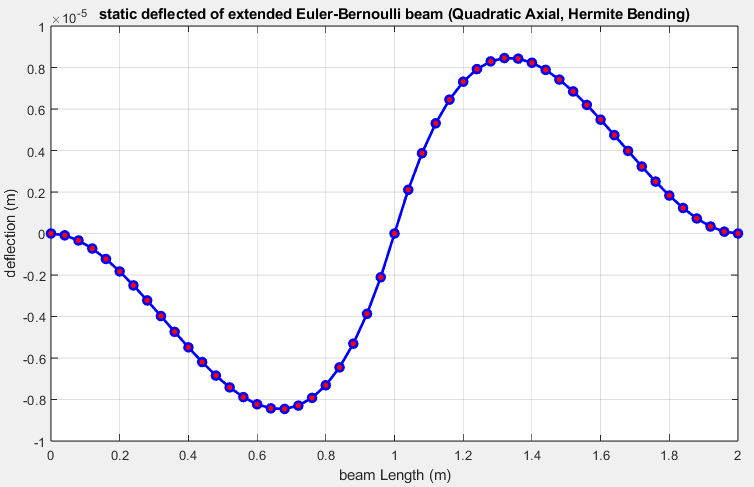
\includegraphics[width=0.8\textwidth]{Quadratic_Axial.png}
		\caption{Schematic of the extended Euler--Bernoulli beam element showing axial and bending DOFs.}
		\label{fig:beam-element}
	\end{figure}
	
	
\end{document}
